\paragraph{Question and motivation.}
Section~4.3 of the paper states that the heap redzone size ``affects the
ability to find heap-buffer-overflow bugs'' and that ``large values may lead
to significant slowdown and increased memory usage, especially if the tested
program allocates many small chunks''. It also attributes most of the memory
overhead (C3) to malloc redzones. Neither statement is backed by data. The
redzone is the main accuracy--cost trade-off a user controls: the paper
evaluates with 32\,B, while its default was 128\,B. We therefore ask how time
and memory scale with the redzone, and whether the sensitivity follows
allocation behaviour.

\paragraph{Design.}
We reuse the \cmd{asan} binaries and the paper's options and change exactly
one factor, the run-time option \cmd{redzone}$\in\{16,32,64,128,256\}$
(minimum heap redzone in bytes). The machine, inputs and binaries stay the
same, and base runs are interleaved with the others (\RzRuns{} repetitions,
\cmd{results/raw/redzone/}).

\paragraph{Results.}
Figure~\ref{fig:rz} and Table~\ref{tab:rz} show the results.
\begin{itemize}
\item \emph{Memory responds strongly.} From 16\,B to 256\,B, the total peak
RSS increase grows from \RzMsixteen$\times$ to \RzMtwofiftysix$\times$. The
growth comes from four programs whose peak heap consists of many small live
objects: \cmd{lua} (\RzMemMostsixteen$\rightarrow$\RzMemMosttwofiftysix$\times$),
\cmd{libxml2} (1.64$\rightarrow$3.44$\times$), \cmd{perl}
(1.13$\rightarrow$3.01$\times$) and \cmd{sqlite} (1.55$\rightarrow$1.96$\times$).
The other \RzMemFlat{} programs change by less than 5\%. The rank correlation
between the rate of small ($\le$64\,B) allocations and the memory growth is
$\rho=\RzMemSpearman$ (Figure~\ref{fig:rz}, right). \cmd{tramp3d} is the main
outlier: it allocates many small objects but frees them quickly, so few of
them are live at the peak.
\item \emph{Time responds weakly.} The average slowdown rises only from
\RzTsixteen$\pm$\RzTsixteensd$\times$ to
\RzTtwofiftysix$\pm$\RzTtwofiftysixsd$\times$, which is comparable to the
run-to-run noise. Only two programs slow down clearly: \cmd{lua}
(\RzMostTsixteen$\rightarrow$\RzMostTtwofiftysix$\times$) and \cmd{libxml2}
(1.85$\rightarrow$2.66$\times$). Their extra time goes into poisoning larger
redzones and touching more memory. For the rest, the differences are within
noise ($\rho=\RzSpearman$ between small-allocation rate and added slowdown).
\end{itemize}

\paragraph{Interpretation.}
The results support Section~4.3 of the paper for memory, and only partly for
time. A larger redzone inflates the programs that keep many small heap objects
live, and it makes only the most allocation-intensive of them noticeably
slower. They also refine C3: redzones are the part of \asan{}'s memory
overhead that grows with the program's small-object heap, while for programs
with large buffers the overhead is fixed and small. The paper measured with
32\,B rather than its default of 128\,B. Under our setup, 128\,B would have
raised the total memory increase from \RzMthirtytwo$\times$ to
\RzMonetwentyeight$\times$, mostly in the malloc-intensive kind of program the
paper singles out (perlbench, xalancbmk). Larger redzones catch overflows that
run further past the end of an object. A user who raises them therefore pays
mainly in memory, and in time only for allocation-heavy code.

\begin{figure}[h]
\centering
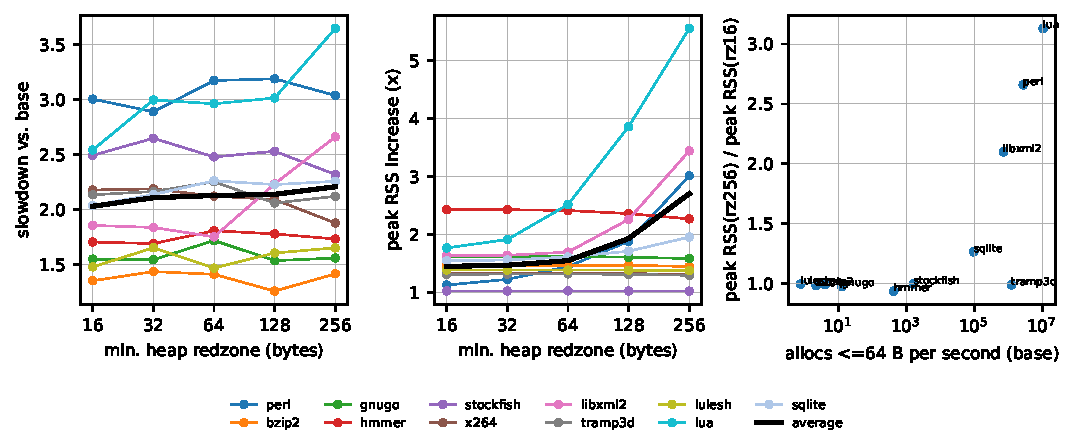
\includegraphics[width=\linewidth]{figures/fig_redzone.pdf}
\caption{Extension: minimum heap redzone vs.\ slowdown (left) and peak-RSS
increase (middle), per program and on average (black). Right: memory
sensitivity (peak RSS at 256\,B divided by that at 16\,B) vs.\ the rate of small
allocations.}\label{fig:rz}
\end{figure}

\begin{table}[h]
\centering\small
\caption{Extension: slowdown (T) and memory increase (M, peak RSS) per
minimum redzone size. Averages: mean $\pm$ s.d.\ over \RzRuns{}
repetitions (T) and ratio of totals (M).}\label{tab:rz}
\begin{tabular}{lrrrrrrrr}
\toprule
Benchmark & T rz16 & T rz32 & T rz64 & T rz128 & T rz256 & M rz16 & M rz128 & M rz256 \\
\midrule
\texttt{perl} & 3.00 & 2.89 & 3.17 & 3.19 & 3.04 & 1.13 & 1.89 & 3.01 \\
\texttt{bzip2} & 1.35 & 1.43 & 1.41 & 1.26 & 1.41 & 1.47 & 1.48 & 1.45 \\
\texttt{gnugo} & 1.55 & 1.54 & 1.72 & 1.53 & 1.56 & 1.63 & 1.61 & 1.59 \\
\texttt{hmmer} & 1.70 & 1.69 & 1.80 & 1.78 & 1.73 & 2.43 & 2.36 & 2.27 \\
\texttt{stockfish} & 2.49 & 2.65 & 2.48 & 2.53 & 2.32 & 1.03 & 1.03 & 1.03 \\
\texttt{x264} & 2.18 & 2.19 & 2.12 & 2.09 & 1.88 & 1.34 & 1.33 & 1.32 \\
\texttt{libxml2} & 1.85 & 1.83 & 1.75 & 2.23 & 2.66 & 1.64 & 2.26 & 3.44 \\
\texttt{tramp3d} & 2.13 & 2.16 & 2.25 & 2.06 & 2.12 & 1.32 & 1.32 & 1.30 \\
\texttt{lulesh} & 1.48 & 1.65 & 1.47 & 1.60 & 1.65 & 1.39 & 1.39 & 1.38 \\
\texttt{lua} & 2.54 & 2.99 & 2.96 & 3.01 & 3.65 & 1.77 & 3.86 & 5.55 \\
\texttt{sqlite} & 2.03 & 2.13 & 2.26 & 2.22 & 2.25 & 1.55 & 1.72 & 1.96 \\
\midrule
Average & 2.03$\pm$0.10 & 2.11$\pm$0.19 & 2.13$\pm$0.11 & 2.14$\pm$0.19 & 2.20$\pm$0.11 & 1.45 & 1.93 & 2.71 \\
\bottomrule
\end{tabular}

\end{table}
